\documentclass{article}

% Requires the official NeurIPS 2026 style file (neurips_2026.sty), from the
% workshop's Overleaf template:
% https://www.overleaf.com/latex/templates/formatting-instructions-for-neurips-2026/bjdwqfdkyftc
% Place neurips_2026.sty in the same directory as this file, or import this
% file's body into that Overleaf template project directly.
\usepackage{neurips_2026}

\usepackage[utf8]{inputenc}
\usepackage[T1]{fontenc}
\usepackage{hyperref}
\usepackage{url}
\usepackage{amsmath,amssymb}
\usepackage{graphicx}
\usepackage{xcolor}
\usepackage{tikz}
\usetikzlibrary{arrows.meta,positioning}
\usepackage{pgfplots}
\pgfplotsset{compat=1.18}
\usepackage{booktabs}
\usepackage{algorithm}
\usepackage{algpseudocode}
\usepackage{enumitem}
\usepackage{natbib}

\definecolor{deepblue}{HTML}{1D4289}
\definecolor{paleblue}{HTML}{DBE7FB}

\title{Cross-Vendor Deception Asymmetry in Multi-Agent LLM Social Deduction Games}

% Anonymized for double-blind review, per workshop policy.
\author{
  Anonymous Author(s) \\
  Affiliation withheld for double-blind review
}

\begin{document}

\maketitle

\begin{abstract}
Prior work evaluating large language models (LLMs) in social deduction games such as Mafia and Werewolf has consistently instantiated every agent from a single model family, leaving open whether deception and detection skill transfer symmetrically across model vendors. We introduce a cross-vendor deception-asymmetry framework built on MafiaSim, a Mafia simulator in which up to fifteen distinct commercial and open-weight model families compete in the same game under a secret-ballot voting mechanic. For every (accuser, deceiver) model pair we compute an opportunity-normalized catch rate directly from already-logged secret ballots, requiring no additional gameplay instrumentation or API calls beyond what the simulator records by default. Applied to nine completed games (323 accuser--deceiver opportunities, 40 catches, an aggregate 12.4\% catch rate), the framework surfaces substantial per-model variation in aggregate detectability (0\%--45\% across models with $\geq$10 opportunities) while showing comparatively little evidence, at this sample size, of accuser-specific asymmetry beyond a deceiver's overall detectability. We release the analysis as an open, game-agnostic command-line tool and discuss confounds, chiefly the entanglement of deception skill with conversational engagement, that must be controlled for before the framework can support stronger causal claims.
\end{abstract}

\textbf{Keywords:} large language models, social deduction games, multi-agent systems, deception detection, heterogeneous agents, Mafia, Werewolf, evaluation methodology

\section{Introduction}
\label{sec:intro}

Social deduction games, including Mafia, Werewolf, and their variants, have become a recurring testbed for evaluating large language models' capacity for strategic communication, deception, and theory of mind, because winning requires players to reason about what other agents believe, to lie convincingly under partial information, and to detect when others are lying \citep{eckhaus2025time,feng2024survey,song2025beyond}. The appeal of these games as a benchmark is structural, not incidental: a social deduction game supplies a built-in, unambiguous scoring signal (who wins), a natural information asymmetry between roles, and a requirement that every utterance be interpretable both at face value and as a possible lie, three properties that are difficult to obtain simultaneously in more open-ended agent evaluations.

Nearly every published study we are aware of, however, instantiates every agent, or every agent but one human player, from a single backbone model, varying at most its size or fine-tuning regime \citep{eckhaus2025time,zhang2025dvm,mittal2026triadic}. This is a reasonable default for isolating the effect of model scale or training procedure, but it leaves an important and, to our knowledge, empirically untouched question: when agents from genuinely different model families, with different pretraining corpora, alignment procedures, and RLHF objectives, play against each other under identical game rules, is deception skill symmetric, or does a given family have a systematic blind spot against a specific other family's persuasive style? The distinction matters practically as well as scientifically. As LLM-based agents are increasingly deployed to negotiate, moderate, or transact with agents from other vendors rather than only with humans or copies of themselves, a documented asymmetry, model A is disproportionately good at deceiving model B specifically, would be a genuinely new category of finding: not a capability gap, but a pairwise compatibility gap invisible to any single-model-family benchmark.

MafiaSim, the simulator underlying this work, already answers a version of this question structurally, and did so for reasons unrelated to deception research. Its player-sampling procedure seats one model per company wherever the roster allows, so that a single game routinely pits Claude, GPT, Gemini, Grok, and open-weight models such as Kimi K2 or Mistral Large against one another under identical game rules; this heterogeneity was originally adopted purely for roster diversity in a leaderboard context, and turns out, on inspection of the resulting logs, to be exactly the substrate a deception-asymmetry study needs. This paper is, in that sense, an analysis built on data the system was already producing for another purpose, rather than an experiment designed from scratch, which is also why we present it as a working technical report rather than a controlled study: the roster, role ratios, and even the set of vendors available changed over the period the underlying games were collected (Section~\ref{sec:discussion-roster}), a form of ecological validity that a purpose-built experiment would not have, at the cost of the tighter controls a purpose-built experiment would.

This paper makes four contributions:
\begin{enumerate}[leftmargin=*]
\item We formalize a cross-vendor deception-asymmetry metric, an opportunity-normalized catch rate defined over ordered (accuser, deceiver) model pairs, computable entirely from data a Mafia simulator already logs for other purposes (Section~\ref{sec:methodology}), requiring no new game mechanic and no additional model calls.
\item We implement it as an open, game-agnostic command-line tool that recomputes the full matrix from logged game transcripts in well under a second, so the analysis stays current as new games accumulate rather than requiring a bespoke run.
\item We report preliminary results from nine real games spanning up to fifteen distinct model vendors, including a full pairwise catch-rate matrix and per-model aggregate detectability rankings (Section~\ref{sec:results}), and we explicitly position this against the closest prior work (Section~\ref{sec:positioning}) to make clear what is and is not incrementally new here.
\item We discuss the confounds, principally the entanglement of deception success with conversational engagement, that limit the causal strength of the current results, and lay out four concrete, already-instrumented next steps to address them (Section~\ref{sec:limitations}).
\end{enumerate}

\textbf{Scope note.} This is a working technical report submitted for early-stage feedback, not a claim of a mature, settled result. Sample sizes are small ($n=9$ games); we treat the results as directional throughout and say so explicitly wherever the data does not support a stronger claim, rather than overstating significance to make the contribution appear more settled than it is.

\section{Related Work}
\label{sec:related}

\subsection{Social Deduction Games as LLM Testbeds}

Werewolf and Mafia have both been used as LLM-agent testbeds. \citet{xu2023exploring} conduct an early empirical study of LLMs playing Werewolf, characterizing failure modes in strategy and persuasion when prompted directly, and a companion line of work by \citet{xu2024language} instead trains Werewolf agents end-to-end with reinforcement learning for strategic play. \citet{light2023text} and \citet{wang2023avalon} study the related deduction game Avalon, the former evaluating off-the-shelf LLMs' tactical play and the latter proposing a recursive-contemplation prompting scheme aimed specifically at countering in-game deception. \citet{eckhaus2025time} study a single asynchronous LLM agent embedded among human Mafia players, focusing on when to speak rather than what to say, and release a 33-game human--AI Mafia corpus. \citet{zhang2025dvm} propose DVM, a reinforcement-learning framework that lets a single agent's Werewolf proficiency be dynamically tuned to a target win rate. \citet{song2025beyond} introduce a two-stage, human-data-grounded evaluation of LLM social deduction play across five social-ability dimensions, finding that roughly half of evaluated models score below 0.50 on strategy alignment with winning human play. \citet{mittal2026triadic} studies multi-hop theory of mind by adding a Jester role, whose win condition is orthogonal to both factions, to Werewolf.

\subsection{Multi-Agent LLM Systems and Simulation}

Beyond games specifically, \citet{park2023generative} demonstrate that populations of LLM agents can sustain believable, emergent social behavior in an open-ended simulated town, establishing much of the architectural template (memory, planning, reflection) that later game-playing agents, including MafiaSim's own private-memory and suspicion-tracking features, draw on. \citet{du2023debate} show that having multiple LLM instances debate and critique each other's answers improves factuality and reasoning even when every instance is the same underlying model, a result whose logic (heterogeneous perspectives improve group reasoning) is suggestive for, but never tested against, genuinely heterogeneous multi-vendor debate. \citet{neuberger2024sauce} contribute SAUCE, an infrastructure layer for orchestrating both synchronous and asynchronous multi-agent LLM conversations, of which MafiaSim's own open-floor discussion mechanic is a specialized instance. \citet{guertler2025textarena} release TextArena, a broader competitive text-game platform for LLM agents that Werewolf-style games are a natural fit for. At larger scale, \citet{bakhtin2022human} combine language generation with explicit strategic planning to reach human-level play in Diplomacy, a seven-player game of alliance, betrayal, and negotiation with no single omniscient narrator, the closest large-scale precedent to a multi-agent LLM system where deception is load-bearing to the win condition itself rather than incidental to it.

\subsection{Theory of Mind and Deception in LLMs}

A separate literature asks whether LLMs represent other agents' beliefs at all, independent of any game. \citet{kosinski2023theory} reports that GPT-family models solve a majority of classic false-belief theory-of-mind tasks, while \citet{ullman2023large} shows that this apparent competence is brittle: trivial perturbations to the same task templates, which do not change the underlying reasoning required, collapse performance. \citet{park2023aideception} survey documented cases of AI systems, including LLMs, engaging in strategic deception across a range of settings, and argue that deception capability is likely to outpace targeted mitigations absent dedicated evaluation infrastructure, a call this paper's deception-asymmetry framework is a narrow, empirical instance of answering for one concrete environment. Outside LLM agents specifically, \citet{ibraheem2022putting} and \citet{deruiter2018mafiascum} both study deception detection directly from Mafia text produced by human players, the latter releasing the MafiaScum human-play corpus that much of the classical (pre-LLM) Mafia deception-detection literature is built on.

\subsection{Positioning Relative to Prior Work}
\label{sec:positioning}

Table~\ref{tab:positioning} summarizes the comparison directly. Across the body of work surveyed above, we find no study that seats more than one or two distinct model families against each other in the same social deduction game, and none that reports a pairwise, per-model-pair deception or detection rate rather than an aggregate win rate or a human-alignment score. The incremental contribution of this paper relative to that literature is therefore not a new agent architecture, a new prompting strategy, or a new dataset in the usual sense; it is the observation that a genuinely heterogeneous multi-vendor roster (already a byproduct of MafiaSim's leaderboard design, not built for this purpose) plus a mechanic that already logs secret ballots for spectator replay (also a pre-existing feature, built for a different reason) together are sufficient to compute a class of result, pairwise cross-vendor deception asymmetry, that no prior single-model-family or human-in-the-loop study could produce even in principle, because that class of result is only defined when at least two distinct, identifiable model families are both present in the same game and their per-round choices are individually attributable. Our contribution is consequently best understood as an analysis layer, not a new agent architecture: it is orthogonal to and compatible with every system surveyed above, and could in principle be applied to any of their logs if ballots or accusations were recorded per-model rather than only in aggregate.

\begin{table}[t]
\centering
\caption{Positioning relative to the closest prior work.}
\label{tab:positioning}
\small
\begin{tabular}{@{}p{2.6cm}p{1.6cm}p{1.6cm}p{1.6cm}p{1.9cm}@{}}
\toprule
Work & Distinct vendors/game & Pairwise deception rate & Secret ballots & Post hoc, zero extra calls \\
\midrule
\citet{eckhaus2025time}  & 1 (+human) & No & No & No \\
\citet{zhang2025dvm}     & 1          & No & No & No \\
\citet{song2025beyond}   & $\leq$2    & No & No & No \\
\citet{mittal2026triadic} & 1         & No & No & No \\
\citet{bakhtin2022human} & 1          & No & N/A & No \\
\textbf{This work}       & \textbf{up to 15} & \textbf{Yes} & \textbf{Yes} & \textbf{Yes} \\
\bottomrule
\end{tabular}
\end{table}

\section{The MafiaSim Environment}
\label{sec:environment}

MafiaSim is a Mafia (Werewolf) simulator that connects to each vendor's API directly through provider-specific HTTP adapters, rather than through a single unifying SDK, so that no single vendor's request or response conventions become the implicit lingua franca every other model is silently normalized toward. It assigns each of $n$ players one of four roles (mafia, detective, doctor, villager) in a ratio following common Mafia convention (roughly one mafia per three to four players). Each night, mafia members privately coordinate a kill by majority vote among themselves; the doctor privately protects one player, including possibly themselves; the detective privately learns one player's exact role, not merely their team. Each day, all living players discuss in an open, turn-polled floor rather than a fixed speaking order, a player is given priority whenever another player addresses them by name, then cast a secret ballot to eliminate one player. A tie at the top of the ballot triggers a public ``showdown'': the tied players each get exactly one turn to make their case, after which the table revotes among only the tied set, repeating until the tie breaks or a round limit is reached.

Beyond the core loop, three engineering properties of MafiaSim are directly relevant to how the analysis in this paper should be read. First, private state is genuinely private: each player's system prompt is rebuilt per call from only that player's own role, its own team's history if it has one, and a private memory the player itself chooses to write and update turn over turn (a free-text note plus a structured per-player suspicion tracker); nothing routes between players except what is logged to the public transcript. Second, spend is bounded and measured, not estimated after the fact: a hard per-game cost cap is checked between phases so a single expensive day cannot run away, and every provider's own reported per-call cost, where available, is accumulated per model, which is what makes it possible to say precisely how much the games underlying this paper's Table~\ref{tab:pairwise} cost to produce (\$4.83 across the full 9-game corpus at the time of analysis, unrelated to the deception metric itself but a byproduct of the same instrumentation). Third, the system is explicitly tuned for multi-vendor robustness rather than single-vendor performance: retries distinguish a genuinely malformed model response from a transient provider-routing failure, and the roster has, over the course of operating it, had specific models disabled for measured reasons (excessive cost share, empty completions from reasoning-token starvation, near-duplicate repeated messages) rather than simply added and left unmonitored, a maintenance posture that matters for interpreting Section~\ref{sec:discussion-roster}'s roster non-stationarity discussion.

Two further properties are load-bearing specifically for this study. First, votes are a secret ballot: the identity behind each vote is written only to a spectator-only log, never surfaced to any player's own prompt, mirroring the norm in most real-world Mafia play that the outcome of a vote is public but the ballot itself is not. Because players cannot observe who voted for whom, the deception-asymmetry analysis in this paper is purely observational and post hoc: no player could have adapted its play to the fact that this analysis would later be run on the ballots, which is precisely the property that gives the metric ecological validity as a measure of real gameplay rather than of gaming an observed metric. Second, seat assignment is vendor-diverse by construction: MafiaSim samples one model per distinct company wherever the roster has enough companies to cover every seat, falling back to an even round-robin only when it does not. At the time of the games analyzed here, the roster spanned Anthropic, OpenAI, Google, xAI, Mistral, DeepSeek, Meta, Alibaba, Cohere, Moonshot, and Zhipu; it has since been expanded to fifteen enabled vendors, discussed further in Section~\ref{sec:discussion-roster}.

\section{Methodology}
\label{sec:methodology}

Let $M$ denote the set of model keys in the roster. For a completed game $g$ and a day-vote round on day $D$, let $A(D)$ be the set of players alive entering that round and $\mathit{Maf}(D) \subseteq A(D)$ the subset who are mafia. For a non-mafia voter $v \in A(D)$ and a mafia player $m \in \mathit{Maf}(D) \setminus \{v\}$, we say $(v,m)$ is an \textit{opportunity}: $v$ had the legal option to cast its ballot for $m$, a genuine mafia player, that round. It is a \textit{catch} if $v$'s actual vote target that round equals $m$.

Opportunities and catches are attributed to model keys, not seats, and summed across every round of every logged game:

\begin{align}
\mathrm{Opp}(a,d) &= \sum_{g,D} \big|\{(v,m) \in \mathrm{opportunities} : \mathrm{model}(v){=}a, \mathrm{model}(m){=}d\}\big| \notag\\
\mathrm{Catch}(a,d) &= \sum_{g,D} \big|\{(v,m) \in \mathrm{catches} : \mathrm{model}(v){=}a, \mathrm{model}(m){=}d\}\big| \notag\\
\mathrm{CatchRate}(a,d) &= \mathrm{Catch}(a,d) \,/\, \mathrm{Opp}(a,d) \notag
\end{align}

$\mathrm{CatchRate}(a,d)$ is accuser model $a$'s detection rate against deceiver model $d$ specifically; $1-\mathrm{CatchRate}(a,d)$ is $d$'s deception success rate against that specific accuser. Algorithm~\ref{alg:matrix} gives the exact aggregation procedure; it is a single linear pass over every logged game's vote rounds, with no dependency between games, so it is embarrassingly parallel and, in practice, recomputes the full matrix from every game logged so far in well under a second on a laptop. The full framework is implemented as a pure function over already-serialized game JSON (Figure~\ref{fig:pipeline}) and ships as a command-line subcommand that recomputes the matrix from every logged game on demand, with an optional minimum-opportunity threshold to suppress pairs too sparse to be informative.

\begin{algorithm}[t]
\caption{Cross-Vendor Deception-Asymmetry Matrix}
\label{alg:matrix}
\begin{algorithmic}[1]
\Require Logged games $G$, each with per-round ballots and each player's $(\mathrm{seat}, \mathrm{role}, \mathrm{model})$
\Ensure Matrix $C$ mapping $(a,d) \mapsto (\mathrm{Opp}, \mathrm{Catch})$
\State $C \gets \{\}$ \Comment{empty dict, default $(0,0)$}
\For{each game $g \in G$}
  \State $P \gets$ seat-to-player map for $g$
  \For{each vote round $(D, \mathrm{votes}) \in g.\mathrm{day\_votes}$}
    \State $\mathit{Maf} \gets \{p \in P : p.\mathrm{role} = \textsc{mafia} \wedge \mathrm{alive\_at}(p, D)\}$
    \If{$\mathit{Maf} = \emptyset$} \textbf{continue} \EndIf
    \For{each $(v, t) \in \mathrm{votes}$} \Comment{voter, target}
      \If{$P[v].\mathrm{role} = \textsc{mafia}$} \textbf{continue} \EndIf
      \For{each $m \in \mathit{Maf} \setminus \{v\}$}
        \State $a \gets P[v].\mathrm{model}$; \, $d \gets P[m].\mathrm{model}$
        \State $C[a,d].\mathrm{Opp} \gets C[a,d].\mathrm{Opp} + 1$
        \If{$t = m$}
          \State $C[a,d].\mathrm{Catch} \gets C[a,d].\mathrm{Catch} + 1$
        \EndIf
      \EndFor
    \EndFor
  \EndFor
\EndFor
\State \Return $C$
\end{algorithmic}
\end{algorithm}

\begin{figure}[t]
\centering
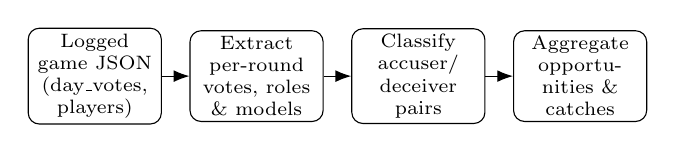
\begin{tikzpicture}[
  node distance=0.35cm,
  box/.style={draw, rounded corners, align=center, font=\scriptsize, minimum height=1.05cm, text width=1.55cm, inner sep=2pt},
  arr/.style={-{Latex[length=2mm]}}
]
\node[box] (a) {Logged game JSON (day\_votes, players)};
\node[box, right=of a] (b) {Extract per-round votes, roles \& models};
\node[box, right=of b] (c) {Classify accuser/ deceiver pairs};
\node[box, right=of c] (d) {Aggregate opportunities \& catches};
\draw[arr] (a) -- (b);
\draw[arr] (b) -- (c);
\draw[arr] (c) -- (d);
\end{tikzpicture}
\caption{The analysis pipeline. Every stage operates on data the simulator already persists for replay and cost-accounting purposes; no gameplay change or extra model call is required to compute or extend the matrix.}
\label{fig:pipeline}
\end{figure}

\section{Experimental Setup}
\label{sec:setup}

We analyze all nine games completed and logged by MafiaSim at the time of writing, spanning eight to fifteen players each, run against the OpenRouter-routed roster over a single development period. Role composition followed the simulator's default ratios (Section~\ref{sec:environment}); temperature was fixed at 0.9 and the per-call token budget at 1400--2000 across the period studied. Across these nine games we observe 92 distinct (accuser, deceiver) model pairs with at least one opportunity, totalling 323 opportunities and 40 catches, an aggregate catch rate of 12.4\%. We emphasize that this figure is a per-ballot rate, not a per-game mafia-loss rate: a table eliminating a mafia player typically requires a plurality, not a single voter's catch, so 12.4\% should not be read as ``mafia lose 12.4\% of the time.''

\section{Results}
\label{sec:results}

Table~\ref{tab:pairwise} reports, for the nine models with the most total opportunity volume, a representative slice of the full pairwise catch-rate matrix, visualized as a heatmap in Figure~\ref{fig:heatmap}. Cell shade is scaled by opportunity count (paler cells have fewer than ten opportunities and should be read cautiously); dashed cells indicate no logged opportunities for that ordered pair; a model paired with itself is marked with a diagonal and excluded, since a model is never asked to accuse itself.

\begin{figure}[t]
\centering
\resizebox{\linewidth}{!}{%
\definecolor{hc0}{HTML}{EAF0F9}
\definecolor{hc1}{HTML}{EAF0F9}
\definecolor{hc2}{HTML}{E7EEF9}
\definecolor{hc3}{HTML}{E3ECFA}
\definecolor{hc4}{HTML}{EEF2F8}
\definecolor{hc5}{HTML}{C9D7EF}
\definecolor{hc6}{HTML}{E7EEF9}
\definecolor{hc7}{HTML}{E7EEF9}
\definecolor{hc8}{HTML}{CCD7EA}
\definecolor{hc9}{HTML}{9FAEC9}
\definecolor{hc10}{HTML}{CBD5E7}
\definecolor{hc11}{HTML}{EAF0F9}
\definecolor{hc12}{HTML}{EAF0F9}
\definecolor{hc13}{HTML}{EAF0F9}
\definecolor{hc14}{HTML}{9FAEC9}
\definecolor{hc15}{HTML}{B8C9E6}
\definecolor{hc16}{HTML}{ECF1F8}
\definecolor{hc17}{HTML}{E1EBFA}
\definecolor{hc18}{HTML}{CBD5E7}
\definecolor{hc19}{HTML}{E7EEF9}
\definecolor{hc20}{HTML}{EEF2F8}
\definecolor{hc21}{HTML}{C8D6F0}
\definecolor{hc22}{HTML}{E1EBFA}
\definecolor{hc23}{HTML}{E7EEF9}
\definecolor{hc24}{HTML}{E7EEF9}
\definecolor{hc25}{HTML}{B5C3DE}
\definecolor{hc26}{HTML}{BEC9DD}
\definecolor{hc27}{HTML}{EEF2F8}
\definecolor{hc28}{HTML}{EAF0F9}
\definecolor{hc29}{HTML}{EEF2F8}
\definecolor{hc30}{HTML}{CDDBF3}
\definecolor{hc31}{HTML}{CCD8EC}
\definecolor{hc32}{HTML}{DDE8FB}
\definecolor{hc33}{HTML}{CBD5E7}
\definecolor{hc34}{HTML}{CCD7ED}
\definecolor{hc35}{HTML}{BEC9DD}
\definecolor{hc36}{HTML}{B7C8E6}
\definecolor{hc37}{HTML}{A4B4CF}
\definecolor{hc38}{HTML}{9DAFD0}
\definecolor{hc39}{HTML}{EEF2F8}
\definecolor{hc40}{HTML}{EEF2F8}
\definecolor{hc41}{HTML}{EEF2F8}
\definecolor{hc42}{HTML}{C2D1EC}
\definecolor{hc43}{HTML}{CCD7EA}
\definecolor{hc44}{HTML}{E5EDF9}
\definecolor{hc45}{HTML}{EEF2F8}
\definecolor{hc46}{HTML}{ECF1F8}
\definecolor{hc47}{HTML}{9FAEC9}
\definecolor{hc48}{HTML}{EEF2F8}
\begin{tikzpicture}[x=0.64cm,y=-0.64cm,every node/.style={font=\scriptsize}]
\node[rotate=60,anchor=west,font=\tiny] at (2.50,-0.15) {Qwen2.5-72B};
\node[rotate=60,anchor=west,font=\tiny] at (3.50,-0.15) {Kimi K2};
\node[rotate=60,anchor=west,font=\tiny] at (4.50,-0.15) {Cl. Haiku 4.5};
\node[rotate=60,anchor=west,font=\tiny] at (5.50,-0.15) {Gemini 3.6 Fl.};
\node[rotate=60,anchor=west,font=\tiny] at (6.50,-0.15) {Command A};
\node[rotate=60,anchor=west,font=\tiny] at (7.50,-0.15) {GPT-5.5};
\node[rotate=60,anchor=west,font=\tiny] at (8.50,-0.15) {Mistral Large};
\node[rotate=60,anchor=west,font=\tiny] at (9.50,-0.15) {DeepSeek Chat};
\node[rotate=60,anchor=west,font=\tiny] at (10.50,-0.15) {Llama 3.3 70B};
\node[anchor=east,font=\tiny] at (1.9,2.10) {Qwen2.5-72B};
\node[anchor=east,font=\tiny] at (1.9,3.10) {Kimi K2};
\node[anchor=east,font=\tiny] at (1.9,4.10) {Cl. Haiku 4.5};
\node[anchor=east,font=\tiny] at (1.9,5.10) {Gemini 3.6 Fl.};
\node[anchor=east,font=\tiny] at (1.9,6.10) {Command A};
\node[anchor=east,font=\tiny] at (1.9,7.10) {GPT-5.5};
\node[anchor=east,font=\tiny] at (1.9,8.10) {Mistral Large};
\node[anchor=east,font=\tiny] at (1.9,9.10) {DeepSeek Chat};
\node[anchor=east,font=\tiny] at (1.9,10.10) {Llama 3.3 70B};
\fill[gray!15] (2.00,1.60) rectangle (3.00,2.60);
\draw[gray!60] (2.00,1.60) -- (3.00,2.60);
\fill[hc0] (3.00,1.60) rectangle (4.00,2.60);
\node[text=black] at (3.50,1.98) {\textbf{0\%}};
\node[text=black,font=\tiny] at (3.50,2.32) {n=3};
\fill[hc1] (4.00,1.60) rectangle (5.00,2.60);
\node[text=black] at (4.50,1.98) {\textbf{0\%}};
\node[text=black,font=\tiny] at (4.50,2.32) {n=3};
\fill[hc2] (5.00,1.60) rectangle (6.00,2.60);
\node[text=black] at (5.50,1.98) {\textbf{0\%}};
\node[text=black,font=\tiny] at (5.50,2.32) {n=4};
\draw[gray!40,dashed] (6.00,1.60) rectangle (7.00,2.60);
\fill[hc3] (7.00,1.60) rectangle (8.00,2.60);
\node[text=black] at (7.50,1.98) {\textbf{0\%}};
\node[text=black,font=\tiny] at (7.50,2.32) {n=6};
\draw[gray!40,dashed] (8.00,1.60) rectangle (9.00,2.60);
\fill[hc4] (9.00,1.60) rectangle (10.00,2.60);
\node[text=black] at (9.50,1.98) {\textbf{0\%}};
\node[text=black,font=\tiny] at (9.50,2.32) {n=1};
\draw[gray!40,dashed] (10.00,1.60) rectangle (11.00,2.60);
\fill[hc5] (2.00,2.60) rectangle (3.00,3.60);
\node[text=black] at (2.50,2.98) {\textbf{11\%}};
\node[text=black,font=\tiny] at (2.50,3.32) {n=9};
\fill[gray!15] (3.00,2.60) rectangle (4.00,3.60);
\draw[gray!60] (3.00,2.60) -- (4.00,3.60);
\fill[hc6] (4.00,2.60) rectangle (5.00,3.60);
\node[text=black] at (4.50,2.98) {\textbf{0\%}};
\node[text=black,font=\tiny] at (4.50,3.32) {n=4};
\fill[hc7] (5.00,2.60) rectangle (6.00,3.60);
\node[text=black] at (5.50,2.98) {\textbf{0\%}};
\node[text=black,font=\tiny] at (5.50,3.32) {n=4};
\draw[gray!40,dashed] (6.00,2.60) rectangle (7.00,3.60);
\fill[hc8] (7.00,2.60) rectangle (8.00,3.60);
\node[text=black] at (7.50,2.98) {\textbf{20\%}};
\node[text=black,font=\tiny] at (7.50,3.32) {n=5};
\draw[gray!40,dashed] (8.00,2.60) rectangle (9.00,3.60);
\fill[hc9] (9.00,2.60) rectangle (10.00,3.60);
\node[text=black] at (9.50,2.98) {\textbf{100\%}};
\node[text=black,font=\tiny] at (9.50,3.32) {n=1};
\draw[gray!40,dashed] (10.00,2.60) rectangle (11.00,3.60);
\draw[gray!40,dashed] (2.00,3.60) rectangle (3.00,4.60);
\fill[hc10] (3.00,3.60) rectangle (4.00,4.60);
\node[text=black] at (3.50,3.98) {\textbf{25\%}};
\node[text=black,font=\tiny] at (3.50,4.32) {n=4};
\fill[gray!15] (4.00,3.60) rectangle (5.00,4.60);
\draw[gray!60] (4.00,3.60) -- (5.00,4.60);
\fill[hc11] (5.00,3.60) rectangle (6.00,4.60);
\node[text=black] at (5.50,3.98) {\textbf{0\%}};
\node[text=black,font=\tiny] at (5.50,4.32) {n=3};
\fill[hc12] (6.00,3.60) rectangle (7.00,4.60);
\node[text=black] at (6.50,3.98) {\textbf{0\%}};
\node[text=black,font=\tiny] at (6.50,4.32) {n=3};
\fill[hc13] (7.00,3.60) rectangle (8.00,4.60);
\node[text=black] at (7.50,3.98) {\textbf{0\%}};
\node[text=black,font=\tiny] at (7.50,4.32) {n=3};
\draw[gray!40,dashed] (8.00,3.60) rectangle (9.00,4.60);
\fill[hc14] (9.00,3.60) rectangle (10.00,4.60);
\node[text=black] at (9.50,3.98) {\textbf{100\%}};
\node[text=black,font=\tiny] at (9.50,4.32) {n=1};
\draw[gray!40,dashed] (10.00,3.60) rectangle (11.00,4.60);
\fill[hc15] (2.00,4.60) rectangle (3.00,5.60);
\node[text=black] at (2.50,4.98) {\textbf{18\%}};
\node[text=black,font=\tiny] at (2.50,5.32) {n=11};
\fill[hc16] (3.00,4.60) rectangle (4.00,5.60);
\node[text=black] at (3.50,4.98) {\textbf{0\%}};
\node[text=black,font=\tiny] at (3.50,5.32) {n=2};
\fill[hc17] (4.00,4.60) rectangle (5.00,5.60);
\node[text=black] at (4.50,4.98) {\textbf{0\%}};
\node[text=black,font=\tiny] at (4.50,5.32) {n=7};
\fill[gray!15] (5.00,4.60) rectangle (6.00,5.60);
\draw[gray!60] (5.00,4.60) -- (6.00,5.60);
\fill[hc18] (6.00,4.60) rectangle (7.00,5.60);
\node[text=black] at (6.50,4.98) {\textbf{25\%}};
\node[text=black,font=\tiny] at (6.50,5.32) {n=4};
\fill[hc19] (7.00,4.60) rectangle (8.00,5.60);
\node[text=black] at (7.50,4.98) {\textbf{0\%}};
\node[text=black,font=\tiny] at (7.50,5.32) {n=4};
\draw[gray!40,dashed] (8.00,4.60) rectangle (9.00,5.60);
\fill[hc20] (9.00,4.60) rectangle (10.00,5.60);
\node[text=black] at (9.50,4.98) {\textbf{0\%}};
\node[text=black,font=\tiny] at (9.50,5.32) {n=1};
\draw[gray!40,dashed] (10.00,4.60) rectangle (11.00,5.60);
\fill[hc21] (2.00,5.60) rectangle (3.00,6.60);
\node[text=black] at (2.50,5.98) {\textbf{10\%}};
\node[text=black,font=\tiny] at (2.50,6.32) {n=10};
\fill[hc22] (3.00,5.60) rectangle (4.00,6.60);
\node[text=black] at (3.50,5.98) {\textbf{0\%}};
\node[text=black,font=\tiny] at (3.50,6.32) {n=7};
\fill[hc23] (4.00,5.60) rectangle (5.00,6.60);
\node[text=black] at (4.50,5.98) {\textbf{0\%}};
\node[text=black,font=\tiny] at (4.50,6.32) {n=4};
\fill[hc24] (5.00,5.60) rectangle (6.00,6.60);
\node[text=black] at (5.50,5.98) {\textbf{0\%}};
\node[text=black,font=\tiny] at (5.50,6.32) {n=4};
\fill[gray!15] (6.00,5.60) rectangle (7.00,6.60);
\draw[gray!60] (6.00,5.60) -- (7.00,6.60);
\fill[hc25] (7.00,5.60) rectangle (8.00,6.60);
\node[text=black] at (7.50,5.98) {\textbf{33\%}};
\node[text=black,font=\tiny] at (7.50,6.32) {n=6};
\draw[gray!40,dashed] (8.00,5.60) rectangle (9.00,6.60);
\fill[hc26] (9.00,5.60) rectangle (10.00,6.60);
\node[text=black] at (9.50,5.98) {\textbf{50\%}};
\node[text=black,font=\tiny] at (9.50,6.32) {n=2};
\draw[gray!40,dashed] (10.00,5.60) rectangle (11.00,6.60);
\draw[gray!40,dashed] (2.00,6.60) rectangle (3.00,7.60);
\fill[hc27] (3.00,6.60) rectangle (4.00,7.60);
\node[text=black] at (3.50,6.98) {\textbf{0\%}};
\node[text=black,font=\tiny] at (3.50,7.32) {n=1};
\fill[hc28] (4.00,6.60) rectangle (5.00,7.60);
\node[text=black] at (4.50,6.98) {\textbf{0\%}};
\node[text=black,font=\tiny] at (4.50,7.32) {n=3};
\draw[gray!40,dashed] (5.00,6.60) rectangle (6.00,7.60);
\draw[gray!40,dashed] (6.00,6.60) rectangle (7.00,7.60);
\fill[gray!15] (7.00,6.60) rectangle (8.00,7.60);
\draw[gray!60] (7.00,6.60) -- (8.00,7.60);
\draw[gray!40,dashed] (8.00,6.60) rectangle (9.00,7.60);
\fill[hc29] (9.00,6.60) rectangle (10.00,7.60);
\node[text=black] at (9.50,6.98) {\textbf{0\%}};
\node[text=black,font=\tiny] at (9.50,7.32) {n=1};
\draw[gray!40,dashed] (10.00,6.60) rectangle (11.00,7.60);
\fill[hc30] (2.00,7.60) rectangle (3.00,8.60);
\node[text=black] at (2.50,7.98) {\textbf{7\%}};
\node[text=black,font=\tiny] at (2.50,8.32) {n=14};
\fill[hc31] (3.00,7.60) rectangle (4.00,8.60);
\node[text=black] at (3.50,7.98) {\textbf{17\%}};
\node[text=black,font=\tiny] at (3.50,8.32) {n=6};
\fill[hc32] (4.00,7.60) rectangle (5.00,8.60);
\node[text=black] at (4.50,7.98) {\textbf{0\%}};
\node[text=black,font=\tiny] at (4.50,8.32) {n=9};
\draw[gray!40,dashed] (5.00,7.60) rectangle (6.00,8.60);
\fill[hc33] (6.00,7.60) rectangle (7.00,8.60);
\node[text=black] at (6.50,7.98) {\textbf{25\%}};
\node[text=black,font=\tiny] at (6.50,8.32) {n=4};
\fill[hc34] (7.00,7.60) rectangle (8.00,8.60);
\node[text=black] at (7.50,7.98) {\textbf{14\%}};
\node[text=black,font=\tiny] at (7.50,8.32) {n=7};
\fill[gray!15] (8.00,7.60) rectangle (9.00,8.60);
\draw[gray!60] (8.00,7.60) -- (9.00,8.60);
\fill[hc35] (9.00,7.60) rectangle (10.00,8.60);
\node[text=black] at (9.50,7.98) {\textbf{50\%}};
\node[text=black,font=\tiny] at (9.50,8.32) {n=2};
\draw[gray!40,dashed] (10.00,7.60) rectangle (11.00,8.60);
\fill[hc36] (2.00,8.60) rectangle (3.00,9.60);
\node[text=black] at (2.50,8.98) {\textbf{19\%}};
\node[text=black,font=\tiny] at (2.50,9.32) {n=16};
\fill[hc37] (3.00,8.60) rectangle (4.00,9.60);
\node[text=black] at (3.50,8.98) {\textbf{67\%}};
\node[text=black,font=\tiny] at (3.50,9.32) {n=3};
\fill[hc38] (4.00,8.60) rectangle (5.00,9.60);
\node[text=white] at (4.50,8.98) {\textbf{50\%}};
\node[text=white,font=\tiny] at (4.50,9.32) {n=6};
\fill[hc39] (5.00,8.60) rectangle (6.00,9.60);
\node[text=black] at (5.50,8.98) {\textbf{0\%}};
\node[text=black,font=\tiny] at (5.50,9.32) {n=1};
\fill[hc40] (6.00,8.60) rectangle (7.00,9.60);
\node[text=black] at (6.50,8.98) {\textbf{0\%}};
\node[text=black,font=\tiny] at (6.50,9.32) {n=1};
\fill[hc41] (7.00,8.60) rectangle (8.00,9.60);
\node[text=black] at (7.50,8.98) {\textbf{0\%}};
\node[text=black,font=\tiny] at (7.50,9.32) {n=1};
\draw[gray!40,dashed] (8.00,8.60) rectangle (9.00,9.60);
\fill[gray!15] (9.00,8.60) rectangle (10.00,9.60);
\draw[gray!60] (9.00,8.60) -- (10.00,9.60);
\draw[gray!40,dashed] (10.00,8.60) rectangle (11.00,9.60);
\fill[hc42] (2.00,9.60) rectangle (3.00,10.60);
\node[text=black] at (2.50,9.98) {\textbf{13\%}};
\node[text=black,font=\tiny] at (2.50,10.32) {n=15};
\fill[hc43] (3.00,9.60) rectangle (4.00,10.60);
\node[text=black] at (3.50,9.98) {\textbf{20\%}};
\node[text=black,font=\tiny] at (3.50,10.32) {n=5};
\fill[hc44] (4.00,9.60) rectangle (5.00,10.60);
\node[text=black] at (4.50,9.98) {\textbf{0\%}};
\node[text=black,font=\tiny] at (4.50,10.32) {n=5};
\fill[hc45] (5.00,9.60) rectangle (6.00,10.60);
\node[text=black] at (5.50,9.98) {\textbf{0\%}};
\node[text=black,font=\tiny] at (5.50,10.32) {n=1};
\fill[hc46] (6.00,9.60) rectangle (7.00,10.60);
\node[text=black] at (6.50,9.98) {\textbf{0\%}};
\node[text=black,font=\tiny] at (6.50,10.32) {n=2};
\fill[hc47] (7.00,9.60) rectangle (8.00,10.60);
\node[text=black] at (7.50,9.98) {\textbf{100\%}};
\node[text=black,font=\tiny] at (7.50,10.32) {n=1};
\draw[gray!40,dashed] (8.00,9.60) rectangle (9.00,10.60);
\fill[hc48] (9.00,9.60) rectangle (10.00,10.60);
\node[text=black] at (9.50,9.98) {\textbf{0\%}};
\node[text=black,font=\tiny] at (9.50,10.32) {n=1};
\fill[gray!15] (10.00,9.60) rectangle (11.00,10.60);
\draw[gray!60] (10.00,9.60) -- (11.00,10.60);
\end{tikzpicture}
}
\caption{Pairwise catch rate, rows = accuser model, columns = deceiver model, for the nine models with the highest total opportunity volume. Percentage is $\mathrm{Catch}(a,d)/\mathrm{Opp}(a,d)$; $n$ is the opportunity count for that pair. Fill shade darkens with $n$ (pale at $n{=}1$, saturated at $n{\geq}10$) so sparse cells visually recede rather than appearing as confidently as well-sampled ones. Dashed outline = no logged opportunities for that ordered pair; diagonal = self-pair, excluded by construction.}
\label{fig:heatmap}
\end{figure}

Two patterns are visible in Figure~\ref{fig:heatmap}. First, the Qwen2.5-72B model is caught infrequently by every accuser with a non-trivial sample against it: 7\% by Mistral Large ($n{=}14$), 11\% by Kimi K2 ($n{=}9$), 13\% by Llama~3.3~70B ($n{=}15$), 18\% by Gemini~3.6~Flash ($n{=}11$), and 19\% by DeepSeek~Chat ($n{=}16$). Second, DeepSeek Chat shows the opposite pattern as a deceiver, caught 50\%--67\% of the time by the (small-$n$) accusers it faced. Aggregated over all accusers, Figure~\ref{fig:barchart} and Table~\ref{tab:aggregate} rank every model by overall detectability as a deceiver.

\begin{figure}[t]
\centering
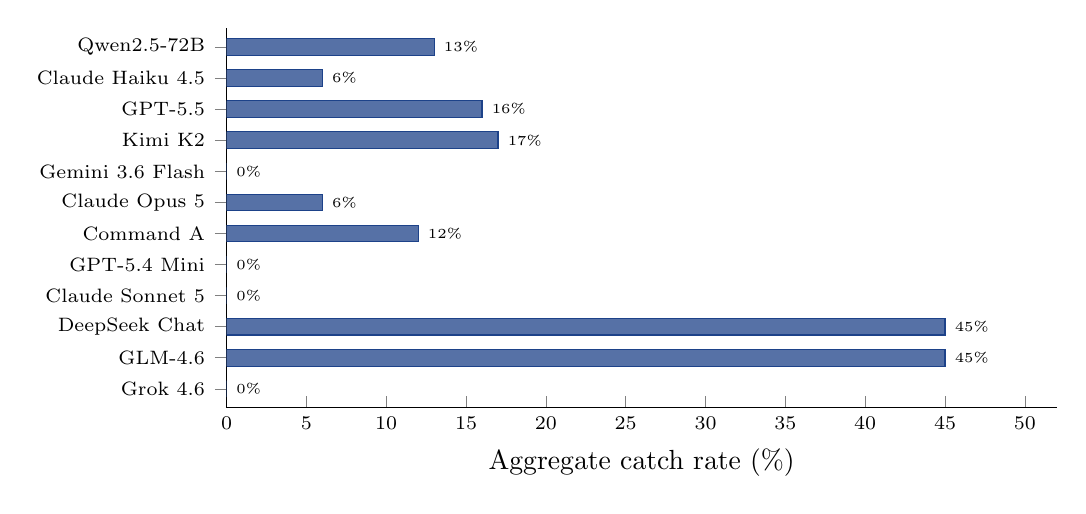
\begin{tikzpicture}
\begin{axis}[
  xbar, y dir=reverse,
  bar width=6pt,
  width=\linewidth, height=6.4cm,
  xmin=0, xmax=52,
  xlabel={Aggregate catch rate (\%)},
  symbolic y coords={Qwen2.5-72B,Claude Haiku 4.5,GPT-5.5,Kimi K2,Gemini 3.6 Flash,Claude Opus 5,Command A,GPT-5.4 Mini,Claude Sonnet 5,DeepSeek Chat,GLM-4.6,Grok 4.6},
  ytick=data,
  nodes near coords={\pgfmathprintnumber{\pgfplotspointmeta}\%},
  every node near coord/.append style={font=\tiny, /pgf/number format/fixed},
  tick label style={font=\scriptsize},
  axis lines*=left,
  enlarge y limits=0.055,
]
\addplot[fill=deepblue!75,draw=deepblue] coordinates {
 (13,Qwen2.5-72B)
 (6,Claude Haiku 4.5)
 (16,GPT-5.5)
 (17,Kimi K2)
 (0,Gemini 3.6 Flash)
 (6,Claude Opus 5)
 (12,Command A)
 (0,GPT-5.4 Mini)
 (0,Claude Sonnet 5)
 (45,DeepSeek Chat)
 (45,GLM-4.6)
 (0,Grok 4.6)
};
\end{axis}
\end{tikzpicture}
\caption{Aggregate catch rate by deceiver model, summed over every accuser. Exact opportunity counts $n$ per model are given in Table~\ref{tab:aggregate}; the two highest bars (DeepSeek Chat, GLM-4.6) rest on only 11 opportunities each and should not be read as more reliable than that small $n$ suggests.}
\label{fig:barchart}
\end{figure}

\begin{table}[t]
\centering
\caption{Pairwise catch rate, core models ($\mathrm{Opp} \geq 9$).}
\label{tab:pairwise}
\begin{tabular}{@{}llrrr@{}}
\toprule
Accuser & Deceiver & Opp & Catch & Rate \\
\midrule
DeepSeek Chat     & Qwen2.5-72B     & 16 & 3 & 19\% \\
Llama 3.3 70B     & Qwen2.5-72B     & 15 & 2 & 13\% \\
Mistral Large     & Qwen2.5-72B     & 14 & 1 & 7\%  \\
Gemini 3.6 Flash  & Qwen2.5-72B     & 11 & 2 & 18\% \\
Command A         & Qwen2.5-72B     & 10 & 1 & 10\% \\
Kimi K2           & Qwen2.5-72B     & 9  & 1 & 11\% \\
Mistral Large     & Claude Haiku 4.5 & 9  & 0 & 0\%  \\
\bottomrule
\end{tabular}
\\[0.3em]
\footnotesize Full 92-pair table reproducible via the released tool at a minimum-opportunity threshold of 1.
\end{table}

\begin{table}[t]
\centering
\caption{Aggregate detectability as deceiver (all accusers).}
\label{tab:aggregate}
\begin{tabular}{@{}lrrr@{}}
\toprule
Model & Opp & Catch & Rate \\
\midrule
Qwen2.5-72B      & 82 & 11 & 13\% \\
Claude Haiku 4.5 & 47 & 3  & 6\%  \\
GPT-5.5          & 43 & 7  & 16\% \\
Kimi K2          & 36 & 6  & 17\% \\
Gemini 3.6 Flash & 18 & 0  & 0\%  \\
Claude Opus 5    & 18 & 1  & 6\%  \\
Command A        & 17 & 2  & 12\% \\
GPT-5.4 Mini     & 16 & 0  & 0\%  \\
Claude Sonnet 5  & 16 & 0  & 0\%  \\
DeepSeek Chat    & 11 & 5  & 45\% \\
GLM-4.6          & 11 & 5  & 45\% \\
Grok 4.6         & 8  & 0  & 0\%  \\
\bottomrule
\end{tabular}
\end{table}

\section{Discussion}
\label{sec:discussion}

\subsection{Detectability appears deceiver-dominant, not pair-specific}

If deception success were strongly asymmetric, a property of the specific (accuser, deceiver) pair driven by e.g. one vendor's writing style exploiting a specific weakness of another's, we would expect a given deceiver's catch rate to vary substantially across different accusers. Qwen2.5-72B's catch rate against the five accusers with $n{\geq}9$ ranges only from 7\% to 19\%, a narrower spread than the 0\%--45\% spread across \textit{different deceivers} in Table~\ref{tab:aggregate}. At this sample size, the dominant source of variation in our data is which model is being accused, not which model is doing the accusing: we find more evidence for a per-model detectability ranking than for true pairwise asymmetry. This does not rule out asymmetry; it means the current data does not yet demonstrate it convincingly, and more opportunities per cell are needed before the pairwise structure in Figure~\ref{fig:heatmap} can be trusted over the marginal ranking in Table~\ref{tab:aggregate}.

\subsection{Deception skill is confounded with engagement}

The metric as defined cannot distinguish a mafia model that is actively and skillfully deflecting suspicion from one that is simply quiet enough to avoid drawing scrutiny in the first place. Both produce a low catch rate. Qwen2.5-72B's low aggregate detectability is consistent with either explanation from vote data alone; distinguishing them requires joining this analysis against MafiaSim's discussion-turn logs (message count, whether the player was directly addressed) as a covariate, data the simulator already records but that this version of the framework does not yet incorporate.

\subsection{Roster non-stationarity}
\label{sec:discussion-roster}

The nine games analyzed here were run over a period during which the roster itself changed: several models present in this dataset have since been disabled in the live roster, for reasons ranging from measured cost dominance to reasoning-token starvation observed independently of this analysis. Seven models added to the roster after these nine games (spanning Amazon, NVIDIA, MiniMax, Microsoft, IBM, Tencent, and Baidu) have zero opportunities in the current matrix, since no game including them has yet completed. The matrix in this paper is a snapshot of a moving roster, not a controlled comparison of the current one.

\section{Limitations and Future Work}
\label{sec:limitations}

The chief limitation is sample size: 323 total opportunities distributed across 92 pairs leaves most individual cells too sparse for a confident pairwise claim, as flagged throughout by shade-scaled figures and explicit $n$ annotations rather than by hiding the uncertainty. We see four concrete next steps. First, run enough additional games, compute budget permitting, to bring the core model pairs in Table~\ref{tab:pairwise} past $n{\approx}30$, and to give the seven newly added vendors their first opportunities. Second, add an engagement-normalized variant of the metric that controls for message volume, isolating deception skill from mere quietness (Section~\ref{sec:discussion}). Third, join this analysis against the structured per-player suspicion tracker MafiaSim now maintains, to test whether a deceiver's catch rate correlates with how often it is \textit{named} in another player's tracker even when not ultimately voted for, a finer-grained signal than the binary vote outcome used here. Fourth, extend the framework beyond votes to the mafia's own private night-chat transcripts (also already logged), to measure whether a model's success at planning a kill correlates with its success at evading day-phase suspicion for that same kill.

\section{Conclusion}
\label{sec:conclusion}

We introduced a cross-vendor deception-asymmetry framework for multi-agent LLM social deduction games, motivated by the observation that the published literature exclusively studies single-model-family tournaments despite the field's rapid diversification into many competing model vendors. The framework is computed entirely from data a Mafia simulator already logs, requires no new gameplay mechanic, and is released as an open command-line tool. Preliminary results from nine games and 323 real accuser--deceiver opportunities show wide variation in per-model detectability (0\%--45\%) but, at this sample size, weaker evidence for accuser-specific asymmetry than for a deceiver-dominant detectability ranking, a finding we report as directional pending more data, in keeping with the scope this report claims for itself.

\bibliographystyle{plainnat}
\begin{thebibliography}{19}

\bibitem[Bakhtin et~al.(2022)]{bakhtin2022human} A.~Bakhtin, N.~Brown, E.~Dinan, G.~Farina, C.~Flaherty, D.~Fried, A.~Goff, J.~Gray, H.~Hu, A.~P.~Jacob, M.~Komeili, K.~Konath, M.~Kwon, A.~Lerer, M.~Lewis, A.~H.~Miller, S.~Mitts, A.~Renduchintala, S.~Roller, et~al. Human-level play in the game of diplomacy by combining language models with strategic reasoning. \textit{Science}, 378:1067--1074, 2022.

\bibitem[de~Ruiter and Kachergis(2018)]{deruiter2018mafiascum} B.~de~Ruiter and G.~Kachergis. The MafiaScum dataset: A large text corpus for deception detection. \textit{arXiv:1811.07851}, 2018.

\bibitem[Du et~al.(2023)]{du2023debate} Y.~Du, S.~Li, A.~Torralba, J.~B.~Tenenbaum, and I.~Mordatch. Improving factuality and reasoning in language models through multiagent debate. \textit{arXiv:2305.14325}, 2023.

\bibitem[Eckhaus et~al.(2025)]{eckhaus2025time} N.~Eckhaus, U.~Berger, and G.~Stanovsky. Time to talk: LLM agents for asynchronous group communication in Mafia games. In \textit{Findings of the Association for Computational Linguistics: EMNLP 2025}, pages 11356--11368, 2025.

\bibitem[Feng et~al.(2024)]{feng2024survey} X.~Feng, L.~Dou, E.~Li, Q.~Wang, H.~Wang, Y.~Guo, C.~Ma, and L.~Kong. A survey on large language model-based social agents in game-theoretic scenarios. \textit{arXiv:2412.03920}, 2024.

\bibitem[Guertler et~al.(2025)]{guertler2025textarena} L.~Guertler, B.~Cheng, S.~Yu, B.~Liu, L.~Choshen, and C.~Tan. TextArena. \textit{arXiv:2504.11442}, 2025.

\bibitem[Ibraheem et~al.(2022)]{ibraheem2022putting} S.~Ibraheem, G.~Zhou, and J.~DeNero. Putting the con in context: Identifying deceptive actors in the game of mafia. In \textit{Proc. Society for Computation in Linguistics}, pages 158--168, 2022.

\bibitem[Kosinski(2023)]{kosinski2023theory} M.~Kosinski. Evaluating large language models in theory of mind tasks. \textit{arXiv:2302.02083}, 2023.

\bibitem[Light et~al.(2023)]{light2023text} J.~Light, M.~Cai, S.~Shen, and Z.~Hu. From text to tactic: Evaluating LLMs playing the game of Avalon. \textit{arXiv:2310.05036}, 2023.

\bibitem[Mittal(2026)]{mittal2026triadic} A.~Mittal. Triadic Werewolf: A Jester role for multi-hop theory of mind in LLMs. \textit{arXiv:2606.27909}, 2026.

\bibitem[Neuberger et~al.(2024)]{neuberger2024sauce} S.~Neuberger, N.~Eckhaus, U.~Berger, A.~Taubenfeld, G.~Stanovsky, and A.~Goldstein. SAUCE: Synchronous and asynchronous user-customizable environment for multi-agent LLM interaction. \textit{arXiv:2411.03397}, 2024.

\bibitem[Park et~al.(2023a)]{park2023generative} J.~S.~Park, J.~C.~O'Brien, C.~J.~Cai, M.~R.~Morris, P.~Liang, and M.~S.~Bernstein. Generative agents: Interactive simulacra of human behavior. \textit{arXiv:2304.03442}, 2023a.

\bibitem[Park et~al.(2023b)]{park2023aideception} P.~S.~Park, S.~Goldstein, A.~O'Gara, M.~Chen, and D.~Hendrycks. AI deception: A survey of examples, risks, and potential solutions. \textit{arXiv:2308.14752}, 2023b.

\bibitem[Song et~al.(2025)]{song2025beyond} Z.~Song, Y.~Huang, J.~Liu, H.~Luo, C.~Wang, L.~Gao, Z.~Xu, M.~Han, X.~Chang, and X.~Chen. Beyond survival: Evaluating LLMs in social deduction games with human-aligned strategies. \textit{arXiv:2510.11389}, 2025.

\bibitem[Ullman(2023)]{ullman2023large} T.~Ullman. Large language models fail on trivial alterations to theory-of-mind tasks. \textit{arXiv:2302.08399}, 2023.

\bibitem[Wang et~al.(2023)]{wang2023avalon} S.~Wang, C.~Liu, Z.~Zheng, S.~Qi, S.~Chen, Q.~Yang, A.~Zhao, C.~Wang, S.~Song, and G.~Huang. Avalon's game of thoughts: Battle against deception through recursive contemplation. \textit{arXiv:2310.01320}, 2023.

\bibitem[Xu et~al.(2023)]{xu2023exploring} Y.~Xu, S.~Wang, P.~Li, F.~Luo, X.~Wang, W.~Liu, and Y.~Liu. Exploring large language models for communication games: An empirical study on werewolf. \textit{arXiv:2309.04658}, 2023.

\bibitem[Xu et~al.(2024)]{xu2024language} Z.~Xu, C.~Yu, F.~Fang, Y.~Wang, and Y.~Wu. Language agents with reinforcement learning for strategic play in the werewolf game. In \textit{Proc. 41st International Conference on Machine Learning (ICML)}, 2024.

\bibitem[Zhang et~al.(2025)]{zhang2025dvm} Z.~Zhang, Y.~Lan, Y.~Chen, L.~Wang, X.~Wang, and H.~Wang. DVM: Towards controllable LLM agents in social deduction games. \textit{arXiv:2501.06695}, 2025.

\end{thebibliography}

\end{document}
